%-*-latex-*-

\begin{center}
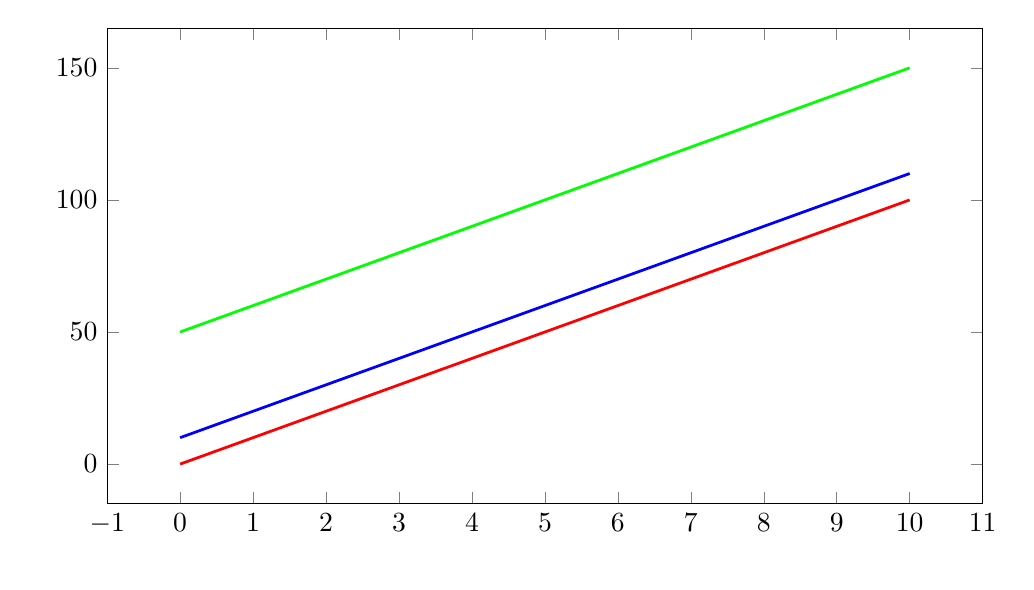
\begin{tikzpicture}[line width=1]
\begin{axis}[width=5in, height=3in,
             scatter/classes={a={mark=*,draw=black}},
             xlabel={\mbox{}},
             xlabel style={name=xlabel}, 
             ylabel={\mbox{}}, 
             legend style={
                at={(xlabel.south)},
                yshift=-1ex,
                anchor=north,
                legend cell align=left,
                },
        ]
]
\addplot[draw=red, line width=1] coordinates {(0.0,0.0)
(5.0,50.0)
(10.0,100.0)
(10.0,100.0)};\addplot[draw=blue, line width=1] coordinates {(0.0,10.0)
(5.0,60.0)
(10.0,110.0)
(10.0,110.0)};\addplot[draw=green, line width=1] coordinates {(0.0,50.0)
(5.0,100.0)
(10.0,150.0)
(10.0,150.0)};
\end{axis}\end{tikzpicture}\end{center}
